\documentclass[dutch,english,whitelogo]{tudelft-report}
\usepackage{changes}
\usepackage{csquotes}
\usepackage{babel}
\usepackage{graphicx}
\graphicspath{ {images/} }
% the syle=apa is only in ShareLatex use 'draft' for WIP
\usepackage[backend=biber,sorting=ynt,style=apa]{biblatex}
\DeclareLanguageMapping{english}{english-apa}
\addbibresource{citations.bib}

% \usepackage{lineno}

\usepackage{enumitem}
\setlist[enumerate]{itemsep=3pt,parsep=3pt}
\setlist[enumerate,2]{topsep=1pt,parsep=2.5pt}

\setlist[itemize]{itemsep=2pt, parsep=2pt}

\setlength\parindent{0pt}

\begin{document}
% 
%% Use Roman numerals for the page numbers of the title pages and table of
%% contents.
\frontmatter

%% Uncomment following 19 lines for a cover with a picture on the lower half only
% \title[tudelft-white]{Title}
% \subtitle[tudelft-cyan]{Optional subtitle}
% \author[tudelft-white]{J.\ Random Author}
% \affiliation{Technische Universiteit Delft}
% \coverimage{cover.jpg}
% \titleoffsetx{10cm}
% \titleoffsety{10cm}
% \afiloffsetx{1cm}
% \afiloffsety{18cm}
% \covertext[tudelft-white]{
%    \textbf{Cover Text} \\
%    possibly \\
%    spanning 
%    multiple 
%    lines
%    \vfill
%    ISBN 000-00-0000-000-0
% }
% \makecover

%% Uncomment following 16 lines for a cover with a picture on the lower half only
\title[tudelft-white]{Plan van aanpak}
\subtitle[tudelft-black]{Ontwikkel een Statistiek platform voor Shop2market}
\author[tudelft-white]{S.\ Oldeman}
\affiliation{HBO-ICT aan Hogeschool Utrecht}
\coverimage{tank.jpg}
\covertext[tudelft-white]{
    \textbf{Hoe kunnen statistieken} \\
     voor Adcurve \\
     actueel blijven en op tijd berekend zijn \\
    
    % \vfill
    % ISBN 000-00-0000-000-0
}
\setpagecolor{tudelft-cyan}
% \makecover[split]


%% Include an optional title page.
\begin{titlepage}


\begin{center}


%% Print the title in cyan.
{\makeatletter
\largetitlestyle\fontsize{64}{94}\selectfont\@title
\makeatother}

%% Print the optional subtitle in black.
{\makeatletter
\ifx\@subtitle\undefined\else
    \bigskip
   {\tudsffamily\fontsize{22}{32}\selectfont\@subtitle}    
\fi
\makeatother}

\bigskip
\bigskip

door

\bigskip
\bigskip

%% Print the name of the author.
{\makeatletter
%\largetitlefont\Large\bfseries\@author
\largetitlestyle\fontsize{26}{26}\selectfont\@author
\makeatother}

\bigskip
\bigskip

ter verkrijging van de graad van Bachalor HBO-ICT

aan de Hoge school Utrecht,

in het openbaar de verdedigen in Juni, 2016.

\vfill

\begin{tabular}{lll}
    Student nummer: & 1571564 \\
    Project duur: & \multicolumn{2}{l}{18 maart 2016 -- 31 mei 2016} \\
    Afstudeer examinatoren:
        & Dhr.\ M.\ Dumont, & HU, docentbegeleider \\
        & Dhr.\ J.\ W.\ Pauw, & HU \\
        & Dhr.\ M.\ Jorissen, & Shop2market
\end{tabular}
%% Only include the following lines if confidentiality is applicable.


%\centering{
\includegraphics{cover/logo_black}}


\end{center}

\begin{tikzpicture}[remember picture, overlay]
    \node at (current page.south)[anchor=south,inner sep=0pt]{
        
\includegraphics{cover/logo_black}
    };
\end{tikzpicture}

\end{titlepage}



\chapter*{Voorwoord}
\setheader{Voorwoord}

Preface\ldots

\begin{flushright}
{\makeatletter\itshape
    \@author \\
    Utrecht, maart 2016
\makeatother}
\end{flushright}



\tableofcontents


%% Use Arabic numerals for the page numbers of the chapters.
\mainmatter

\linenumbers


\chapter{Opdracht}

In dit hoofdstuk wordt beschreven bij welke organisatie de opdracht zich afspeelt. Wat waren de ontwikkelingen binnen de organisatie en wat zijn de redenen om een nieuw project te starten.

\section{Achtergrond}

Het bedrijf Shop2market is een software development bedrijf in de business-to-business sector. Het bedrijft heeft een missie om bedrijven te helpen de winst uit online advertentie campagnes te maximaliseren. 
Voor alsnog diende shop2market als een IT oplossing ondersteunend aan het adviesbedrijf. Het merendeel van deze klanten waren webwinkels in het A segment. Maar omdat de integratie met een webwinkel vaak maatwerk opleverde, duurde een integratie gemiddeld zes tot acht maanden. Hieruit valt ook te concluderen dat veel bedrijven niet de technologische middelen in huis hebben om zelfstandig te kunnen starten met adverteren.

Daarom werd in begin 2015 gestart met de ontwikkeling van een nieuwe dienst: Adcurve. Met alle ervaring vanuit de adviesorganisatie zijn veel processen vertaald naar functionaliteiten. Door de div. functionaliteiten\footnote{ Denk hierbij aan datavisualiasties en beheeracties, soms ook wel "Actionable insights" genoemd.} in Adcurve kan de webwinkeleigenaar zijn online marketing campagnes controleren en binnen budget houden. Dit is mogelijk doordat Adcurve een partij is tussen de webwinkel en publishers. Door platform zoals SEOShop of Magento is het mogelijk webwinkels binnen enkele minuten te integreren. 
Op basis van verzamelde gegevens zoals afkomstige bezoeken, bestellingen en de advertentiekosten worden de nodige statistieken berekend. Met deze gegevens wordt de winstgevendheid per advertentie berekend.


Dit alles heeft als gevolg dat Shop2market nu webwinkels in het midden en klein bedrijf  bedient, maar internationaal op een veel groter volume. Webwinkels zijn nu binnen enkele minuten geïnstalleerd en kunnen hun producten gemakkelijk adverteren via zogeheten publishers. Deze kan de gebruiker zelf installeren binnen Adcurve waar het proces geautomatiseerd word afgehandeld. Publishers zijn de bedrijven die de advertenties publiceren. De soort advertenties verschillen nogal per publisher. Denk bijvoorbeeld aan ingekochte zoekresultaten, producten op prijsvergelijkers of affiliaties, maar ook producten op marktplaatsen.


\pagebreak

\section{Aanleiding} % de aanleiding tot de opdracht

Het afgelopen jaar zijn de meeste basis functionaliteiten voor Adcurve ontwikkeld. Daarnaast zijn er vijf publishers geintegreerd waarvoor een volledige dataintegratie plaatsvindt. Bij deze publishers worden kosten niet door ons berekend o.b.v. een percentage of vast bedrag. De kosten die in rekening zijn gebracht worden gerapporteerd en door Adcurve geïmporteerd.
Omdat de belangrijkste functionaliteiten berusten op de beschikbaarheid van statistieken ligt dit proces aan de kern van de dienst. Helaas verloopt het importeren niet altijd zonder fouten. Het actief bewaken van datakwaliteit is hierdoor een prioriteit geworden. In de huidige situatie is dit nog lastig, doordat het berekenen van de statistieken een langdurig proces is.

De huidige strategie is om meer klanten aan te trekken door meer landen en industriën te ondersteunen. Het is te verwachten dat het aantal data integraties met publishers zal toenemen, en het probleem daardoor groter wordt. Daarnaast is de huidige situatie niet optimaal om mee te beginnen. De statistieken zijn s'middags pas beschikbaar, wardoor veel functionaliteiten werken met data van meer dan een dag oud. Er is hierdoor een een toenemende wens ontstaan om de huidige oplossing te herzien. Dit moet internationale groei van Adcurve onderstuenen, en ruimte bieden om functionaliteiten betrouwbaarder en te maken.

\section{Organisatie} % beschrijving van de organisatie van de opdrachtgever en de plaats van de student daarin

Shop2market is met een team tussen de 10 en 20 werknemers gevestigd in Hilversum. De organisatie kan naar de theorie van
\autocite{mintzberg} worden omschreven als een Adhocracy: “Door de innovatieve aard van projecten is een organisatie gebaat bij flexibiliteit. Een formele hiërarchische structuur werkt daardoor minder goed.” Dit is herkenbaar en valt terug te leiden naar de professionele houding die van werknemers word verwacht. Er word autonomie gegeven om zelf structuur aan te brengen wanneer dit nodig is.

\begin{figure}[h]
    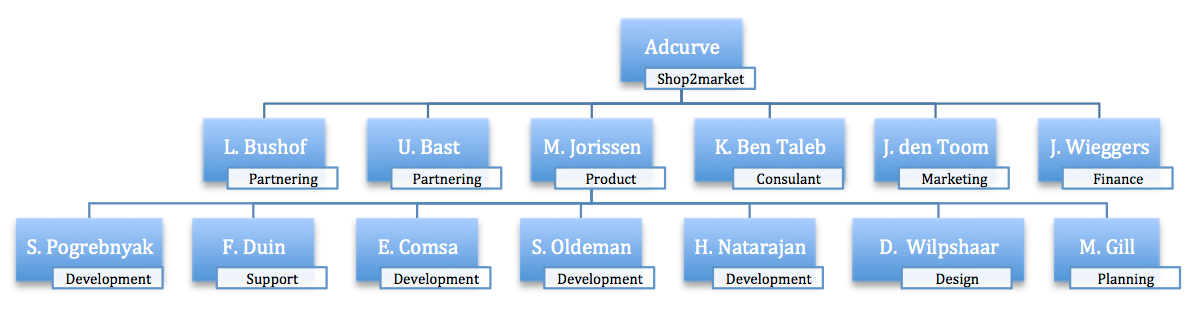
\includegraphics[width=1\textwidth]{organisation_structure.png}
    \caption{Organogram waarin het team en de relaties binnen Shop2market worden afgebeeld.}
    \label{fig:orgchart}
\end{figure}

\pagebreak

\section{De kwestie} % een kwestie (aanleiding, het op te lossen probleem, de te vervullen behoefte of de te benutten kans);

Zoals te lezen valt in de de aanleiding zijn meerdere redenen voor dit project.

\begin{enumerate}
    \item De tijd die het kost om statistieken te berekenen is aan de hoge kant. De berekeningen worden uitgevoerd met behulp van MongoDb MapReduce. Het team voorziet dat deze technologie niet genoeg schaalbaarheid bied. Dit omdat rekentijd linear is toegenomen in relatie tot de hoeveelheid data. Met de verwachte groei van Adcurve komen nieuwe requirements aan het licht en er moet naar een nieuwe oplossing worden gezocht.
    \item Bij voorkeur worden publishers geintegreerd met behulp van API's oftewijl; een externe databron. Op deze manier worden berekeningen uitgevoerd met preciese advertentiekosten. Maar doordat externe factoren nu een rol spelen in de berekeningen is het niet te garanderen dat de de uitkomst altijd correct is. Zodra fouten intern of extern hersteld zijn worden berekeningen voor een bepaalde dag, webwinkel of publisher opnieuw uitgevoerd. Het uitvoeren van dit soort correcties zijn tijdrovend door de huidge implementatie en gebruikte technieken.
    \item Als laatste onstaat er een kans door de huidige problematiek op te lossen. Webwinkels ontvangen tot soms tot 30 dagen na een bestelling een retournering van een of meerdere producten. Dit betekend dat een product niet verkocht is en de omzet uit de bestelling lager ligt dan is berekend. Het is wenselijk om berekende statestieken met betrekken tot retour bestellingen opnieuw te berekenen.
\end{enumerate}


\section{Doelstellingen} % de doelstellingen (wat moet na afloop van het afstudeerproject zijn bereikt);

In het kort moeten webwinkeleigenaren in staat zijn om beslissingen te maken op basis van correcte en actuele gegevens in Adcurve. Dit betekend dat de gegevens die Adcurve toont altijd te verklaren zijn en overeenkomen met de werkelijkheid. Als voorbeeld hiervan zijn gegevens over de vorige dag voor kantooruren beschikbaar en worden retouropdrachten ook verwerkt in Adcurve. Als laatste moeten gegevens accuraat en betrouwbaar zijn, tenzij anders vermeld staat. Daarom moet tijdig herstel van fouten mogelijk zijn.

\section{Type opdracht}

Aan de hand van beschikbare technieken wordt er gekozen een aantal mogelijk oplossingen\newline te proberen middels een Proof of Concept. Dit sluit goed aan bij de aard van een onderzoeksopdracht. Door dit onderzoek moet duidelijk gaan worden: hoe de opdracht kan worden opgelost, of dit mogelijk is en wat er nodig is om de oplossing naar productie te brengen. Door de opdrachtgever is gevraagd om een aantal POC's te ontwikkelen om tot een inzicht over de oplossing te komen. Er is hierdoor sprake van een ontwikkel opdracht.



\chapter{Onderzoeksplan}
% de onderzoeksvragen, hoofdvraag met daaruit voortvloeiende deelvragen die moeten worden beantwoord

In de kwestie zijn de problemen - beter uitdagingen te noemen - omschreven. Omdat een oplossing niet voor de hand ligt, wordt er een onderzoek opgesteld. De leidende hoofdvraag wordt in dit hoofdstuk helder.

\section{Onderzoeksvragen}
Gedurende de uitvoering van de opdracht wordt de volgende hoofdvraag beantwoord: \\
{\large \textit{"Hoe verzorgt een nieuwe implementatie voor het up-to-date houden van statistieken in Adcurve zodat gegevens altijd te verklaren zijn?"}} \\

Om de hoofdvraag te beantwoorden zijn de volgende deelvragen geformuleerd:
\begin{enumerate}
\item Wat zijn de functionele en niet functionele eisen waaraan de oplossing moet voldoen?
\item Wat zijn toonaangevende methodes en technologieën om statistieken te berekenen, die zowel passen bij de wensen en eisen van de opdracht?
\begin{enumerate}
    \item Hoe kan de opdracht worden opgelost?
\end{enumerate}
\item Welke scenario's komen met regelmaat voor waardoor gegevens niet te verklaren zijn?
\begin{enumerate}
    \item Wat zijn de gerelateerde technische factoren waardoor de scenario's voor verhindering zorgen in de huidige situatie?
    \item Wat zijn de mogelijke strategieën en technieken om dit op te lossen?
\end{enumerate}

\item Wat zijn de gepresenteerde oplossingen en waarom zijn deze volledig of niet?
\end{enumerate}

\section{Literatuur} %  (optioneel) een beschrijving van de belangrijkste literatuur die onderzocht zal worden

Voorbeelden van mogelijk jargon die zullen voorkomen in de thesis zijn data aggregaties, data transformaties en het selecteren en installeren van big data tools. Deze concepten worden onderlegd door onder andere de volgende literatuur:

\begin{itemize}
    \item Data Mining, Concepts and Techniques \parencite{data-mining}
    \item I <3 Logs, Event data, stream processing, and data integration \parencite{logs}
    \item Fast Data Processing with Spark \parencite{spark}
    \item Real-Time Big Data Analytics \parencite{realtime-architectures}
\end{itemize}

Tijdens de selectie wordt mogelijk gebruik gemaakt van verschillende fases uit “de Berenschot-methode” \parencite{cuppen}.
Daarnaast zal tijdens het voeren van gesprekken, interviews en presentaties binnen de organisatie mogelijk gebruik worden gemaakt van de theorie uit “Adviseren als tweede beroep, resultaat bereiken als adviseur” \parencite{adviseren}.

\newpage

\section{Onderzoek methode} % de te gebruiken methoden/technieken/middelen (ook van het onderzoek) en, indien van toepassing, de

% \section{Deelvragen} deelvragen voorkomend uit de gekozen ontwerpmethode (optioneel);

Voor qualitatief onderzoek wordt een \textit{Case studie} gebruikt om de problemen in de gegeven context te analyseren. Methodes binnen dit type onderzoek zijn: explanatory, descriptive en exploratory. \parencite{john-dudovskiy}. Het onderzoek is ontworpen om de fases van een Case study uit te voeren. Het ontwerp is omschreven in tabel \ref{tab:onderzoekmethode}.

\begin{center}
\begin{table}[bh]
% \centering
\caption{Onderzoek methodes met te gebruiken methoden/technieken/middelen per deelvraag}
\label{tab:onderzoekmethode}
\def\arraystretch{1.5}
\begin{tabular}{|l|p{4cm}|p{2cm}|p{2.5cm}|p{4.5cm}|}
\hline
% \rowcolor{lightgray} 
\textbf{\#} & \textbf{Deelvraag} & \textbf{Type vraag} & \textbf{Methode} & \textbf{Actie / Resultaat} \\
\hline
1 & Wat zijn de functionele en niet functionele eisen, waaraan de oplossing moet voldoen?
  & Descriptive
  & Interviews
  & MosCow prioriteiten lijst en checklist samenstellen \\
\hline
2 & Wat zijn toonaangevende methodes en technologieën om statistieken te berekenen, en passen bij de wensen en eisen van de opdracht?
  & Descriptive
  & Literature-\newline research
  & Analyseren van bronnen m.b.v. van checklist wordt een shortlist samengesteld  \\
\hline
3 & Welke scenario's komen met regelmaat voor waardoor gegevens niet te verklaren zijn?
  & Descriptive
  & Interviews,\newline Literature-\newline research
  & Inventariseren op te lossen scenario 's met prioriteit d.m.v. Impact analysis \\
\hline
3a & Wat zijn de gerelateerde technische factoren waardoor de scenario's voor verhindering zorgen in de huidige situatie?
   & Descriptive
   & Literature-\newline research
   & Vergelijkingstabel huidige en wenselijke situatie met daarbij de technissche afhankelijkheden om een scenario te kunnen voorkomen \\
\hline
3b & Wat zijn de mogelijke strategieën en technieken om dit op te lossen?
   & Designing
   & Interviews,\newline Literature-\newline research
   & Door het toepassen van de vergelijkingstabel met gevonden technologieën worden mogelijke oplossingen ontworpen \\
\hline
4 & Wat zijn de mogelijke oplossingen en hoe wordt dit gevalideerd?
   & Comparative
   & Literature-\newline research,\newline group-discussion
   & Door het Analyseren van mogelijke ontwerpen en groep discussie worden er een beperkt aantal Proof of Concepts geformuleerd met eisen. \\
\hline
5 & Wat zijn de gepresenteerde oplossingen en waarom zijn deze volledig of niet?
  & Explanatory
  & Case study
  & Conclusies op basis van van verzamelde gegevens tijdens POC fase, zoals bijv. performance tests. Tabel van oplossingen met theorieën die het resultaat verklaren. \\
\hline
\end{tabular}
\end{table}
\end{center}

\chapter{Planning} % de projectactiviteiten met een beschrijving van de onderlinge samenhang, de mijlpalen en een fasering in de tijd met een schatting van de te besteden uren voor de verschillende uit te voeren activiteiten;

\section{De opdracht} % de afstudeeropdracht met mogelijke deelopdrachten, met vermelding van de projectgrenzen en randvoorwaarden en, indien het afstudeerproject onderdeel uitmaakt van een groter project, de afbakening t.o.v. het grotere project;

\section{De projectorganisatie} % de projectorganisatie;

    \subsection{Organisatie structuur}

    De software ontwikkeling valt onder leiding van M. Jorissen. In nauwe samenwerking met M. Gill zijn zij verantwoordelijk voor de project analyse en planning. Het development team bestaat uit zes ontwikkelaars waaronder één ontwerper D. Wilpshaar.
    De architectuur wordt geleid door S. Pogrebnyak. Dit team is verantwoordelijk voor het uitwerken en oplossen van projecten. Hierbij word gebruik gemaakt van een aantal methodieken en gewoontes vanuit Agile-softwareontwikkeling, waaronder: Kanban, Daily standup, Retrospectives, Extreme Programming (XP), Test Driven Development (TDD) en Continuous integration (CI).

    \subsection{Werkwijze en methodieken}

    Ondanks dat er in de werkwijze vaak een uitgebreide planning of requirements analyse ontbreekt, word de productiviteit en software kwaliteit toch bewaakt door de principes uit XP zoals TDD. Refactoring speelt hier een grootte rol in.\parencite{refactoring-ruby}
    \footnote{“Code refactoring is het proces waarbij de structuur van bestaande code word gewijzigd zonder de functionaliteit te wijzigen”…“dit komt ten goede aan de onderhoudbaarheid van code, en creëert nieuwe architectuur of object modellen om code makkelijker te kunnen uitbreiden met nieuwe functionaliteiten“}.
    Hierdoor kan het team zich veroorloven om bij het ontwerpen en ontwikkelen van projecten minder vooruit te plannen. Software word hierdoor gevormd door de requirements voor die in huidige situatie aanwezig zijn. In tegenstelling tot het ontwikkelen met abstracties zodat software flexibel genoeg is voor latere aanpassingen en requirements. Veel planning is hierdoor niet aanwezig en technische implementatie komt vooral tot stand door TDD, brainstorm sessies. Dit is mede mogelijk doordat de omgeving de mogelijkheid bied om fouten te maken.

    \subsection{Project verantwoordlijkheden}

    Het plannen en ontwikkelen van het software project omschreven in dit documet valt onder de volledige verantwoordelijkheid van de student. De doelstellingen en requirements worden in overleg met M. Jorissen vastgelegd. In verband met overdracht en kennis deling zal er afstemming plaats vinden met S. Pogrebnyak technische aspecten. Bijvoorbeeld over de aansluiting op huidige visie en de productie omgeving en mogelijke aanpassingen of toevoegingen aan de infrastructuur.
    De student ziet het als zijn verantwoordelijkheid is om op innovatieve wijze software te ontwikkelen.


\section{Activiteiten} % de projectactiviteiten met een beschrijving van de onderlinge samenhang, de mijlpalen en een fasering in de
tijd met een schatting van de te besteden uren voor de verschillende uit te voeren activiteiten;

\section{Risico's} % de eventuele risico’s met maatregelen;

\section{Oplevering}
% twee data voor het inleveren van concepten van de scriptie (circa 6 resp. 3 weken voor de inleverdatum van

de definitieve versie van de scriptie);


%% Use letters for the chapter numbers of the appendices.
\appendix

%\input{appendix-a}

\printbibliography

\end{document}